% arara: pdflatex
% arara: bibtex
% arara: pdflatex
% arara: pdflatex
% 
% Annual Cognitive Science Conference
% Sample LaTeX Paper -- Proceedings Format
% 

% Original : Ashwin Ram (ashwin@cc.gatech.edu)       04/01/1994
% Modified : Johanna Moore (jmoore@cs.pitt.edu)      03/17/1995
% Modified : David Noelle (noelle@ucsd.edu)          03/15/1996
% Modified : Pat Langley (langley@cs.stanford.edu)   01/26/1997
% Latex2e corrections by Ramin Charles Nakisa        01/28/1997 
% Modified : Tina Eliassi-Rad (eliassi@cs.wisc.edu)  01/31/1998
% Modified : Trisha Yannuzzi (trisha@ircs.upenn.edu) 12/28/1999 (in process)
% Modified : Mary Ellen Foster (M.E.Foster@ed.ac.uk) 12/11/2000
% Modified : Ken Forbus                              01/23/2004
% Modified : Eli M. Silk (esilk@pitt.edu)            05/24/2005
% Modified : Niels Taatgen (taatgen@cmu.edu)         10/24/2006
% Modified : David Noelle (dnoelle@ucmerced.edu)     11/19/2014

%% Change "letterpaper" in the following line to "a4paper" if you must.
 
\documentclass[10pt,letterpaper]{article}
 
\usepackage{hyperref}
\usepackage{cogsci}
\usepackage{pslatex}
\usepackage{amsfonts}
\usepackage{graphicx}
\usepackage{apacite}
\usepackage{color}
\usepackage{todonotes}
\usepackage{dsfont}
\usepackage{textcomp}

\definecolor{Red}{RGB}{255,0,0}
\newcommand{\red}[1]{\textcolor{Red}{#1}}

\newcommand{\jd}[1]{\green{$^*$}\marginpar{\footnotesize{JD: \green{#1}}}}

\newcommand{\subsubsubsection}[1]{{\em #1}}
\newcommand{\eref}[1]{(\ref{#1})}
\newcommand{\tableref}[1]{Table \ref{#1}}
\newcommand{\figref}[1]{Figure \ref{#1}}
\newcommand{\appref}[1]{Appendix \ref{#1}}
\newcommand{\sectionref}[1]{Section \ref{#1}}

\title{Why do you ask? Good questions provoke informative answers.}
 
\author{{\large \bf Robert X.~D.~Hawkins, Andreas Stuhlm\"uller, Judith Degen, Noah D.~Goodman}\\
  \{rxdh,astu,jdegen,ngoodman\}@stanford.edu\\
  Department of Psychology, 450 Serra Mall \\
  Stanford, CA 94305 USA}


\begin{document}

\maketitle

\begin{abstract}
What makes a question useful? What makes an answer appropriate? In this paper, we formulate a family of increasingly  sophisticated models of question-answer behavior within the Rational Speech Act framework. We compare these models based on three different pieces of evidence: first, we demonstrate how our answerer models capture a classic effect in psycholinguistics showing that an answerer's level of informativeness varies with the inferred questioner goal, while keeping the question constant. Second, we jointly test the questioner and answerer components of our model based on empirical evidence from  a question-answer reasoning game. Third, we examine a special case of this game to further distinguish among the questioner models. We find that sophisticated pragmatic reasoning is needed to account for some of the data. People can use questions to provide cues to the answerer about their interest, and can select answers that are informative about inferred interests.

\textbf{Keywords:} 
language understanding; pragmatics; Bayesian models; questions; answers
\end{abstract}

\section{Introduction}
\label{sec:intro}

% TODO:
% * think of other good discussion points

\begin{quote}
Q:``Are you gonna eat that?''
A:``Go ahead.''
\end{quote}
In this (real life) example, Q strategically chooses a question that differs from her true interest, avoiding an impolite question, yet manages to signal to A what her interests are; A in turn reasons beyond the overt question and provides an answer that addresses Q's interests.
This subtle interplay raises two questions for formal models of language:
What makes a question useful? What makes an answer appropriate? 
\red{RDH: I commented out a bunch here that was restating the abstract... Might put back in if we have enough space}
%In this paper, we present three progressively more sophisticated computational models of question-answer behavior.
%, which formalize and probe the way answerers infer intentions and the way questioners signal them. 
%We compare these models on the basis of a simulation of a classic question-answer phenomenon and two experiments in which participants must ask and answer questions in a communication game where we can experimentally manipulate the available questions and answers.
%We find that sophisticated pragmatic reasoning is needed to account for some of the data. This suggests that people are able to engage in such reasoning when it is beneficial: they can use questions to provide cues to the answerer about their interest, and can select answers that are informative about inferred interests.

%A:"can you pass he salt?"
%B:"yes (i am able)."

A number of studies in psycholinguistics have provided evidence that answerers are both sensitive to a questioner's goals and attempt to be informative with respect to those goals.
For instance, in the classic study of \citeA{Clark79_IndirectSpeechActs}, researchers called liquor merchants and opened the conversation with one of two sentences to set context: ``I want to buy some bourbon'' (the \emph{uninformative} condition) or ``I've got \$5 to spend'' (the \emph{literal} condition). They then asked, ``Does a fifth of Jim Beam cost more than \$5?'' Merchants gave an exact price significantly more often in the uninformative context than the literal context, where a `yes' or `no' answer was more common. 
In the former case, the merchant inferred that the questioner's goal was just to buy whiskey, so the exact price was the maximally relevant response. In the latter case, the merchant inferred that the questioner's goal was to find out whether or not they could afford the whiskey, hence a simple `yes'  sufficed \cite{Clark79_IndirectSpeechActs}. 
Context and questioner goals have also been implicated in accounts of answers to identification questions like ``who is X?'' \cite{BoerLycan75_KnowingWho}, and to questions like ``where are you?'' that permit answers at many levels of abstraction \cite{Potts12_CardsDialogueCorpus}. While most of this work has focused on \emph{answerer} behavior, it suggests that the question itself is important in prompting a relevant answer.


%Suppose your friend asks you, ``Who is coming to the concert tonight?'' How do you respond? You certainly don't need to give the full list of attendees -- most of whom you do not know -- even though they would all technically be valid answers. Instead, you might only mention the set of \emph{mutual acquaintances} you know are planning to come, assuming that your friend doesn't care about the rest of the crowd. Now, imagine a different scenario. Suppose that you're waiting in line at the box office and want to find out whether your acquaintances had tickets as well. What question would you ask to the person in the ticket booth? If you asked, ``Who is coming to the concert tonight?''  you would likely get a quizzical look and an answer like ``A lot of people, why?'' because the person at the booth does not know your friends or your reason for asking the question. Instead, you might have to directly ask about your friends. Whether you're asking or answering questions, you must engage in some reasoning about the other person's intentions and knowledge. 
%
%Since both questioners and answerers appear to be acutely sensitive to one another's intentions and knowledge, what makes a question useful? What makes an answer to a question useful? In this paper, we present three progressively more sophisticated computational models of question-answer behavior, which formalize and probe this deep interaction between the way answerers infer intentions and the way questioners signal them. We compare these models on the basis of two simulations of classic question-answer phenomena and one experiment in which participants must ask and answer questions given a fixed set of goals. We find that a sophisticated pragmatic answerer is needed to account for the data, and close by proposing that the purpose of questions in dialogue is to provide cues to the answerer about the questioner's goals and intentions.

%A number of studies in psycholinguistics have provided evidence that answerers are both sensitive to a questioner's goals and attempt to be informative with respect to those goals. For example, when people are asked `Do you have the time?'' they typically round their answers to the nearest 5 or 10 minute interval, even when they're wearing a digital watch \cite{DerHenstCarlesSperber02_RelevanceTellingTime}. However, if the question is preceded by the statement ``My watch stopped,'' people make their response precise to the minute  \cite{GibbsBryant08_OptimalRelevance}. While an approximate time is sufficiently informative with respect to most goals, like making it to a meeting on time, this experiment demonstrated that answerers were able to infer that the goal of setting a watch required more precise information.

%Similar evidence comes from a classic study where researchers called liquor merchants and opened the conversation with one of two sentences: "I want to buy some bourbon'' (the `uninformative' condition) or ``I've got \$5 to spend'' (the `literal' condition) They then asked, ``Does a fifth of Jim Beam cost more than \$5?'' Merchants gave an exact price significantly more often in the `uninformative' context than the `literal' context, where a `yes' or `no' answer was more common. In the former case, the merchant inferred that the questioner's goal was just to buy whiskey, so the exact price was the maximally relevant response. In the latter case, the merchant inferred that the questioner's goal was literally to find out whether or not they could afford the whiskey, hence a simple `yes'  sufficed \cite{Clark79_IndirectSpeechActs}. Context and questioner goals have also been implicated in accounts of identification questions like ``who is X?'' \cite{BoerLycan75_KnowingWho}, and to questions like ``where are you?'' that permit answers at many levels of abstraction \cite{Potts12_CardsDialogueCorpus}. While most of this work has focused on \emph{answerer} behavior, it suggests that the question itself can signal the questioner's goals.

\red{RDH: Want to motivate RSA a bit more? We've got some space!}
In addition to these psycholinguistic developments, recent work on Rational Speech Act (RSA) models \cite{frank2012, GoodmanStuhlmuller13_KnowledgeImplicature} has mathematically formalized verbal pragmatic reasoning as a form of rational recursive Bayesian inference, where speakers choose utterances that maximize a particular utility function (dependent on the listener's expected information gain). In this paper we extend the RSA framework to address asking questions and giving answerers. The first challenge is that the speaker utility in this framework is usually identified with information provided---since questions don't provide direct information, we must say what utility they do have. 

We suggest, following \citeA{VanRooy03_QuestioningDecisionProblems}, that the value of a question is the extent to which it can be expected to elicit information relevant to the questioner later in the dialogue. 
More specifically, for the questioner, the value of a question is the expected information she gains about her interests, given the set of likely answers that may be provided by the answerer. 
This requires us to specify a model of the answerer---which can serve as both the model assumed by a questioner, and as a model of answer behavior itself. We explore three, increasingly sophisticated, answerer models. The simplest answerer provides a literal answer to the question (without attempting to be informative);   
the explicit answerer attempts to be informative with respect to the explicit question asked (without inferring the questioner's underlying interests);  
the pragmatic answerer infers the most likely true interests of the questioner, and then informatively addresses those interests.

%In particular, we compare a pragmatic answerer making inferences about the questioner's goals to two simpler models: one that takes into account only that an answerer wants to be maximally informative with respect to the explicit question asked (without inferring the questioner's underlying decision problem) and one that provides a literal answer to the question (without attempting to be maximally informative).  


%% I think we need to discuss at least one previous model, to make it clear why the problem we're tackling is a problem in the first place. The rest can be in related work at the end.
%Recent formal models of question-answer pragmatics have made progress by formally specifying the questioner's goals and what it means for an answerer to be informative with respect to them. van Rooy \citeyear{VanRooy03_QuestioningDecisionProblems}, for instance, defines a goal as a utility function defining a decision problem faced by the questioner. A useful answer under this decision theoretic account is one that maximizes the expected value of the questioner's utility by reducing their uncertainty about the true state of the world. A useful question is one that allows for a sufficiently fine-grained set of answers, optimally distinguishing the worlds relevant to their decision problem. While this framework elegantly accounts for the context-dependence and relevance-maximization of question and answer behavior, it assumes that the questioner's decision problem is known \emph{a priori} by the answerer or fully determined by context. This minimizes the role of the questioner; they just establish a space of answers and then let the answerer do the rest of the work. If the answerer is so adept at using context to determine the relevant information, though, why does the questioner need to ask a question in the first place? Is it just a formality, to prompt the other for their information, or does it serve as a signal in itself, as the studies above suggest? 
%
%We claim that the questioner must reason about answerer behavior, in order to determine what question will produce the most useful answers. This raises a further issue: what kind of answerer does the questioner reason about, and is this internal model accurate? 

The rest of this paper is structured as follows. First, we specify a family of questioner and answerer agents, highlighting some points of divergence from previous RSA models. 
We then formally individuate literal, explicit, and pragmatic models in this family, which represent different hypotheses about how questioners and answerers reason about their task. 
%In particular, we compare a pragmatic answerer making inferences about the questioner's goals to two simpler models: one that takes into account only that an answerer wants to be maximally informative with respect to the explicit question asked (without inferring the questioner's underlying decision problem) and one that provides a literal answer to the question (without attempting to be maximally informative).  
We show that models in this family can accommodate some classic psycholinguistic phenomena related to answerer behavior.
We then use a communication game paradigm that allows us to manipulate the goals, potential questions, and potential answers, testing the predictions of the different models. 
%We find that the most sophisticated, pragmatic models best account for human performance.
%derive predictions for a  of experiments using a novel guessing-game task, and compare these predictions to human performance. 
%In one phase of the task, we require participants to ask a question (from a fixed set of possible questions), given a decision problem. In the second phase, we require participants to give an answer (from a fixed set of possible answers) to a question (from a fixed set of possible questions). 
We close with a brief discussion of related models and future directions.
%These models and data, combined with the psycholinguistic data above, seeks to place question-answer behavior in the larger class of social behavior governed by theory of mind.

\section{A Rational Speech Act model of question and answer behavior}
\label{sec:model}

How should a questioner choose between questions?
%
We start by assuming that the questioner aims to \emph{learn information relevant to a private goal}.
%
In order to choose a question that results in useful information, the questioner reasons about how the answerer would respond, given different possible states of the world, and selects a question that results in an answer that tends to provide goal-relevant information.
%

% This is a divergence from previous RSA models, where agents choose utterances with the goal of imparting information about the state of the world.

More formally, suppose there is a set of world states $\mathcal{W}$, a set of possible goals $\mathcal{G}$, a set of possible questions $\mathcal{Q}$, and a set of possible answers $\mathcal{A}$.
These sets are taken to be in common ground between the questioner and the answerer.
An informational goal $g \in \mathcal{G}$ is a projection function that maps a world state to a particular feature or set of features that the questioner cares about; this is similar to the notion of a QUD (Question Under Discussion) \cite{Roberts96_InformationStructureDiscourse}.
We will use the notation $P_{g}(w)$ to indicate the probability $\hat{P}(g(w))$ of the $g$-relevant aspect of $w$ under the projected distribution 
$\hat{P}(v) = \int_{\mathcal{W}} \delta_{v=g(w)}P(w)dw$.
% Each of these projections corresponds to a different utility function, in a decision-theoretic formulation.
%In order to learn information about their private goal $g$, the questioner reasons about how an internal model of an answerer would respond given some true world.

\newcommand{\KL}[2]{\ensuremath{D_{KL}({#1}\, \| \, {#2})}}
\newcommand{\E}[2]{\ensuremath{\mathbb{E}_{#1}\left [#2 \right]}}

The \textbf{questioner} takes a goal $g \in \mathcal{G}$ as input and returns a distribution over questions $q \in \mathcal{Q}$:
%
$$ 
P(q|g) \propto e^{\E{P(w)}{\KL{P_g(w^*|q, w)}{P_g(w^*)}} - C(q)} 
$$
%
It trades off the cost of asking a question, $C(q)$, and expected information gain. The cost likely depends on question length, among other factors. Information gain is measured as the Kullback-Leibler divergence between the prior distribution over worlds relevant to the goal value, $P_g(w^*)$, and the posterior distribution one would expect after asking a question $q$ in true world state $w$:
%
$$ P_g(w^*|q, w) = \sum_{a \in \mathcal{A}} P(a| q, w)P_g(w^{*}|q, a) $$
%
%This conditional distribution reflects the fact that the answerer (who knows the true world state $w$) may behave noisily, have a limited set of possible answers, or other limitations.
%to questioner (who is inferring a world state $w^*$) is affected by stochastic answerer behavior and a limited set of possible answers. 
This distribution has two components: 
First, it depends on $P(a | q, w^*)$, a model of the answerer which we will explore shortly.
Second, it depends on (the goal projection of) $P(w | q, a)$, an `interpreter' that specifies the likelihood assigned to different worlds given question and answer pairs.

To define the interpreter function, which all agents use to compute the literal interpretation of a question-answer pair, we must assign a semantic meaning to a question.
We assume that a question is an informational goal: a projection from worlds to some aspect of interest. This is equivalent to the more common partition semantics of \citeA{GroenendijkStokhof84_SemanticsOfQuestions}, as can be seen by considering the pre-image of such a projection.
% \red{JD: how can we see this, exactly?} \red{RDH: we say this in the next sentence, right? $q^{-1}(a)$ gives the cell of the partition corresponding to the given aspect of interest\dots}
An answer is then a possible value of the projection function (which picks out an element of the partition via $q^{-1}(a)$).
%The explicit question can be assigned a literal meaning which is a projection from worlds to answer values (this is equivalent to the common partition semantics of questions \cite{gronendijk}).
% likelihood of a world given a question and an answer.
%For the purposes of this paper, we will use Groenendijk \& Stokhof semantics \citeyear{GroenendijkStokhof84_SemanticsOfQuestions}, where a question induces a partition $\mathcal{P}_q$ over the space of possible world and each cell of this partition is an equivalence class corresponding to a different answer. An answer, then, selects a cell of this partition, denoted by $\mathcal{P}_q(a)$, which is a set.
The \textbf{interpreter} constrains the prior on worlds to the subset of its support that is consistent with the semantics of a question-answer pair:
%
$$P(w | q, a) \propto P(w) \delta_{q(w)=a}$$



We next describe three answerer models that embody different assumptions that the questioner could make. All answerers take a question $q \in \mathcal{Q}$ and a world state $w \in \mathcal{W}$ as input and return a distribution over answers $a \in \mathcal{A}$.

The \textbf{literal answerer} simply chooses answers by trading off prior answer probability  and how well a question-answer pair conveys the true state of the world to an interpreter:
%
$$P(a | q,w^*) \propto P(a) P(w^* | q, a) $$
%
For a fixed question, this is equivalent to the speaker in previous RSA models.

The \textbf{explicit answerer} acts like the literal answerer, but evaluates answers with respect to how well they address the explicit question $q$, which can also serve as a projection:
%% FIXME: restrict to truthful answers
%
$$P(a | q, w^*) \propto P(a) P_q(w^* | q, a) $$

The \textbf{pragmatic answerer} also evaluates answers with respect to how well they convey the goal, but doesn't take the question's explicit meaning at face value. Instead, the pragmatic answerer reasons about which goals $g$ are likely given that a question $q$ was asked, and chooses answers that are good on average:
%% FIXME: restrict to truthful answers
%
$$
P(a | q, w^*) \propto p(a) \sum_{g \in \mathcal{G}} P(g|q) P_g(w^*|q, a)
$$
Reasoning backwards from questions to goals is a simple Bayesian inversion of the (explicit) questioner using a prior on goals:
$$
P(g|q) \propto P(q|g)P(g)
$$

For all of the questioner and answerer models, we can vary how strongly optimizing they are---that is, to what extent they are sampling from the distributions defined above, and to what extent they deterministically choose the most likely element. For any such distribution $P$, we introduce an optimality parameter $\alpha$ and transform it as follows:
%
$$ P'(x) \propto e^{\alpha \log(P(x)) } $$
%

This concludes our specification of the model space, giving a set of three answerers and three corresponding questioners that reason about them. We have implemented these models in WebPPL, a probabilistic programming language \cite{GoodmanStuhlmuller14_DIPPL}. The model predictions shown throughout the rest of the paper are computed using this implementation.

\section{Whiskey pricing: a case study}

In order to establish that the proposed model can in principle produce answers that are either over- or under-informative with respect to an explicitly asked question via inference about an underlying questioner goal, we apply the model to Clark's \citeyear{Clark79_IndirectSpeechActs} whiskey study. Recall that in this study, liquor merchants were more likely to give over-informative answers (specifying exact price) to the question ``Does a fifth of Jim Beam cost more than \$5?'' given an \emph{uninformative} context (``I want to buy some bourbon'')  than given a \emph{literal} context (``I've got \$5 to spend''). %The purpose of this application is to examine whether the model can produce answers to the same question that vary in informativeness--not because the question does not matter, but because the inferred questioner goal differs across contexts.

%The same question can evoke different answers, depending on context, and these answers are often over- or under-informative relative to the explicit question. The answerer in these cases is not ignoring the question: the answer is relevant in some way to the question.
%Clark \citeyear{Clark79_IndirectSpeechActs}, demonstrated that context providing indirect evidence for a questioner goal can shift answerer behavior in this way. The question ``Does Jim Beam cost more than \$5?'' was asked prefaced with one of two context sentences, either ``I'd like to buy some whiskey.'' or ``I only have \$5 to spend.'' In the latter case, merchants gave the (over-informative) exact price of liquor more frequently.
%In the following, we illustrate how our modeling framework can accommodate this answerer behavior.

Our world state is a pair of one of $10$ prices (\$1, \$2, \dots, \$10), and a Boolean indicating whether the merchant takes credit cards. There are three possible goals: learning the price of whiskey, learning whether the price is greater than \$5, and learning whether they take credit cards. The set of answers includes exact prices as well as ``yes'' and ``no'', with an answer prior that prefers ``yes''and ``no'' to the exact price answers.

We model the context sentence as affecting the answerer's goal prior. We assume that there is a fixed 40\% probability of the credit card goal, with the remaining 60\% split between the two price-related goals. When the context is ``I'd like to buy some whiskey.'', we assume that the split is even. When it is ``I only have \$5 to spend.'', we assume that it is 9:1 in favor of learning whether the price is greater than \$5.

\subsubsection{Results} When the question is ``Do you take credit cards?'', the pragmatic answerer prefers to give the accurate Boolean answer (with probability $.76$ to $.78$, weakly depending on context), with no preferential treatment for any of the numeric answers. When the question is ``Does Jim Beam cost more than \$5?'', the correct Boolean answer is still the most probable choice, but more weakly (at probability $.44$ to $.49$). Critically, there is a context-dependence for answers to this question: when prefaced with ``I'd like to buy some whiskey.'', the correct exact price answer is favored more strongly (at probability $.18$) than when the context is ``I only have \$5 to spend.'' (probability $.11$). By contrast, the explicit answerer (which has no natural way to account for context) does not make differential predictions in the two situations. %\red{JD: how much depends on the actual chosen values? Can we put in a footnote that convinces us that the numbers  are reasonable or in which way the results vary, if they do?}

This suggests that our pragmatic \emph{answerer} is consistent with human behavior in psychologically interesting situations; that is, the pragmatic answerer component of the model passes the first, qualitative, test. However, we have not yet shown that the \emph{questioner} behavior matches that of humans. Indeed, the questioner has been largely neglected in studies of answering \cite<but see, e.g.,>{Potts12_CardsDialogueCorpus}, even though, as our opening example illustrates, the choice of question is important for understanding answers. In the next section we introduce an experimental paradigm that allows us to explore quantitative behavior of both questioners and answerers.

\begin{figure}
\begin{center}
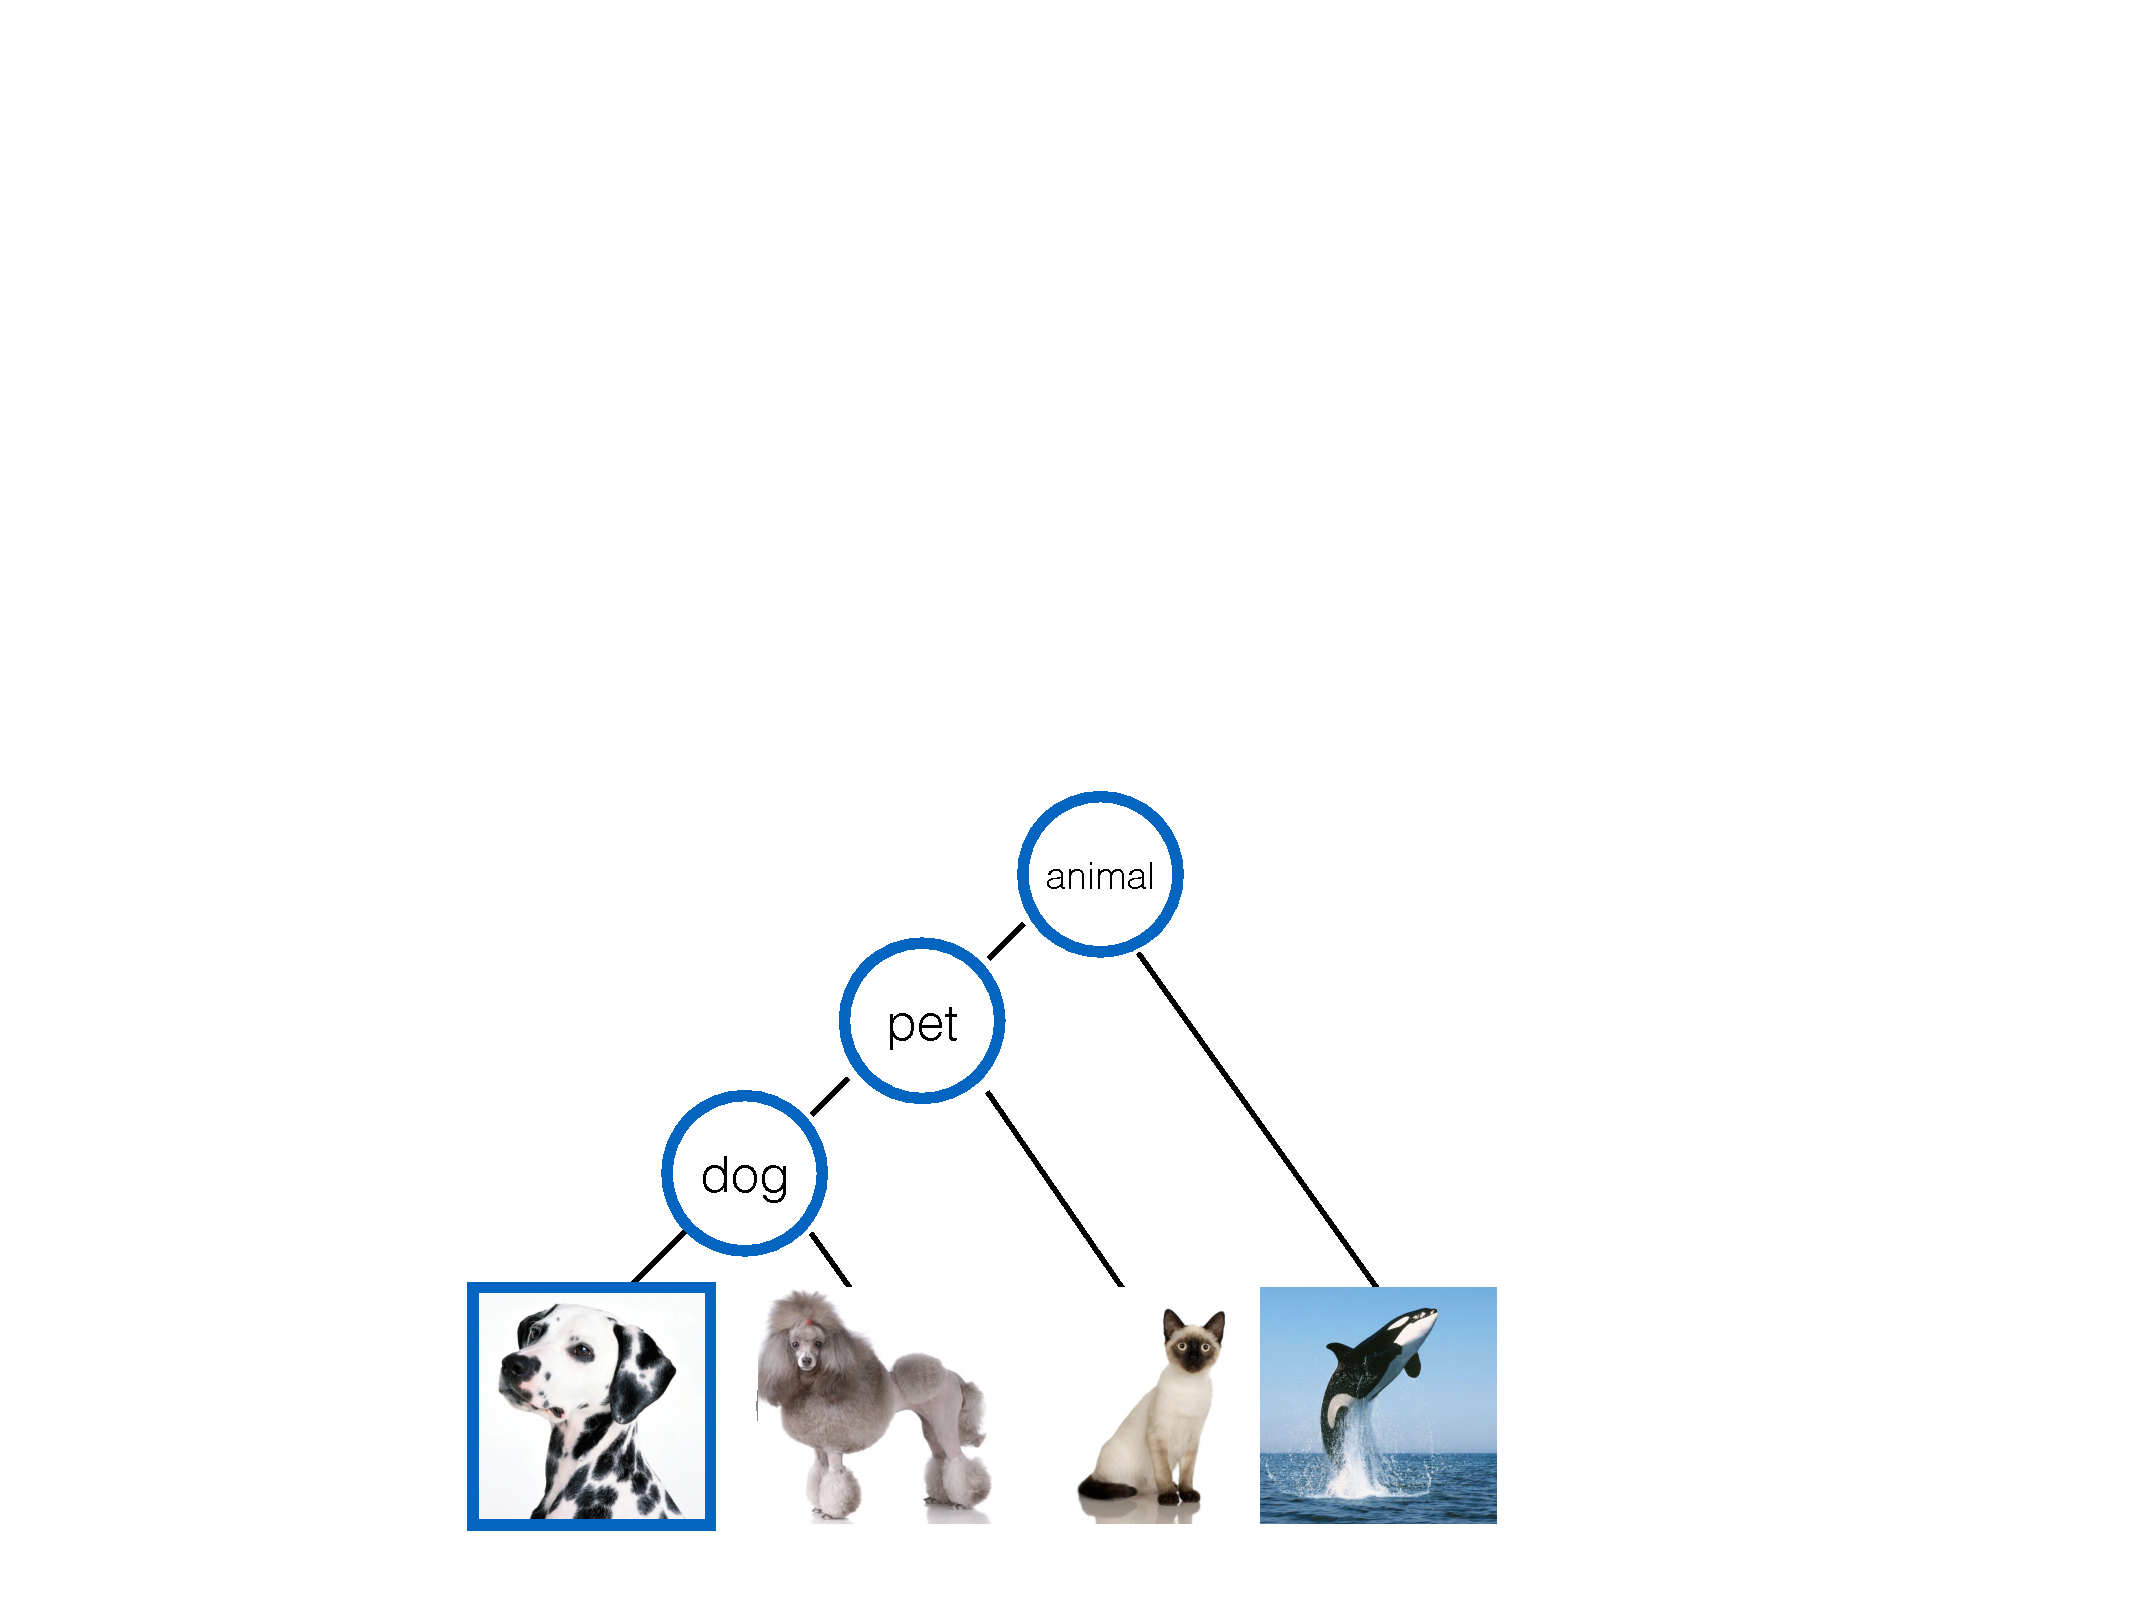
\includegraphics[scale = .35]{taskhierarchy.pdf}
\end{center}
\vspace{-.5cm}
\caption{Stimulus hierarchy used in Exp.~1. The goal space and answer space contained the four leaves. %hidden behind gates (the nodes of the tree). 
The question space, however, was restricted to the highlighted nodes, proceeding up the hierarchy.}
\label{fig:taskhierarchy}
\end{figure}

%\vspace{-1em}

\section{Exp.~1: Hierarchical questions and answers}

	\begin{figure*}[t!]
\begin{center}
\includegraphics[scale = .4]{pragmatic_questioner.pdf}
\includegraphics[scale = .4]{pragmatic_answerer.pdf}
\end{center}
\vspace{-.75cm}
\caption{Exp.~1 results, compared with the predictions of the best-performing model  for questioner (left) and answerer (right).  The explicit and pragmatic questioner do not differ in this task, but the pragmatic answerer better accounts for the qualitative patterns in the response data than the explicit answerer.}
\label{fig:exp1res}
\end{figure*}

 In order to simultaneously test how questioners choose questions when faced with a particular goal and how answerers respond  under uncertainty about this goal, we designed a guessing-game task played by two players: a questioner and an answerer. In this game, $4$ animals (a dalmatian, a poodle, a cat, and a whale) were hidden behind $4$ gates. These animals correspond to different levels in a class hierarchy (see Fig.~\ref{fig:taskhierarchy}). The questioner received a private goal of finding one of the objects (e.g. `find the poodle'), and the answerer (but not questioner) knew the location of each object. Before choosing a gate, the questioner asked the answerer a single question, chosen from a restricted set of options, and the answerer responded by revealing the object behind a single gate. 
 
 This set of restricted options is critical to distinguishing between the pragmatic and explicit variants of our model. Suppose `poodle?' was not available the questioner. If the questioner asks about a `dog?', the poodle and dalmatian would be considered equally good options by an explicit answerer. However, the pragmatic answerer could reason that if the questioner was truly interested in the location of the dalmatian, they would have \emph{asked} about the dalmatian. Because they didn't, they must be interested in the other valid response that they don't have a direct question for: the poodle. 

\subsubsection{Participants} We recruited 125 participants %between the ages of 20 and 75 
from Amazon's Mechanical Turk to participate in this task.  %They were compensated 50\textcent \, for their work, and the median completion time was 3.75 minutes. 
Eleven participants were excluded due to self-reported confusion about the task instructions.

\subsubsection{Stimuli \& Procedure} In terms of our model specification, the world space $\mathcal{W}$ was the set of $4! = 24$ possible assignments of four objects to four gates. The goal space $\mathcal{G}$ was the set of four objects that the questioner could be trying to find (the leaves of the tree in Fig.~\ref{fig:taskhierarchy}). The answer space $\mathcal{A}$ was the set of four gates that the answerer could  reveal. The restricted question space $\mathcal{Q}$ contained the set of highlighted nodes in the hierarchy: `dalmatian?', `dog?', `pet?', and `animal?'. 

Each participant provided responses for four trials in the role of the questioner (corresponding to the four goals), and four trials in the role of the answerer (corresponding to the four possible questions). In the questioner block, players were presented with a private goal from $\mathcal{G}$, like ``find the poodle!'' and prompted to select a question from a drop-down menu containing elements of $\mathcal{Q}$ that would best help them find it. In the answerer block, players were shown which items were behind which gates and were told that the other player had asked a question from $\mathcal{Q}$. They were prompted to select a gate from a drop-down menu that would be most helpful for the questioner, keeping in mind their constraints. 
(To minimize learning effects, questioners did not receive answers and neither role saw the outcome of the game.%; this may have affected motivation.
)
In order to collect responses for all elements of $\mathcal{G}$ and $\mathcal{Q}$, the order of� the questioner and answerer blocks was randomly assigned for each participant, and the order of stimuli within these blocks was also randomized\footnote{The experiment is online at \url{http://cocolab.stanford.edu/cogsci2015/Q_and_A/experiment1/experiment1.html}}. 

\subsubsection{Results}
%\red{check for effect of Q/A block order.}
Results for the questioner role are shown alongside model predictions in Fig.~\ref{fig:exp1res} (left). We find that questioners systematically prefer different questions given different goals, even as those questions become less explicitly informative. $\chi^2$ tests over each of the four response distributions show a significant divergence from uniform. Questioners preferentially ask about the `dalmatian' given the  dalmatian goal, ${\chi^2(3) = 137}, {p < .001}$, about the `dog' given the poodle goal, ${\chi^2(3) = 152}, {p <.001}$, about the `pet' given the cat goal, ${\chi^2(3) = 120},  {p <.001}$, and about the `animal' when given the whale goal, ${\chi^2(3) = 150}, {p <.001}$. This pattern broadly shows that questioners choose the lowest node in the question hierarchy that contains their goal item. 

Results for the answerer role are shown in Fig.~\ref{fig:exp1res} (right). Answerers are highly sensitive to the constraints of the questioner, giving information about the dalmatian when asked about a `dalmatian', ${\chi^2(3) = 281}, {p <.001}$, about the poodle when asked about a `dog', ${\chi^2(3) = 137}, {p <.001}$, about the cat when asked about a `pet', ${\chi^2(3) = 57}, {p<.001}$, and about the whale when asked about an `animal', ${\chi^2(3) = 121}, {p < .001}$. Note that, under an explicit interpretation of the question, revealing the dalmatian and the poodle would both be perfectly acceptable answers to a question about a `dog', but answerers strongly prefer to give the location of the poodle.  In the next section, we compare these results to the predictions of our family of models (Fig. \ref{fig:model_space}). 

\subsubsection{Model comparison}
%\red{check model section to make sure we clearly lay out the agent terminology used here.}

We can rule out both the literal answerer and literal questioner. The \emph{literal answerer} yields a uniform distribution over the four answers %that are the case in the given world. 
This has consequences for the corresponding \emph{literal questioner} model: when this questioner reasons about which question would generate the most helpful answer from the literal answerer, it finds no differences in response probabilities, and thus has no preference for a question. The predictions of this model, plotted against our empirical results, are shown in the left-hand column of Fig. \ref{fig:model_space}; questioners and answerers behave very differently than predicted by these literal models, so we will not consider them further.

The two remaining questioner models make roughly the same predictions for this task, and we are not able to distinguish them on the basis of these data. 
%Since the explicit questioner is nested two levels inside the pragmatic questioner, and each agent in the pragmatic questioner's recursion could in principle be associated with a free rationality parameter, we must consider model complexity when making comparisons. 
To ensure equal footing for the different models, we use just two rationality parameters: one shared by questioners at all levels of recursion, and one shared by answerers at all levels of recursion. 
For each model, we tune these parameters to maximize the correlation between model and data. This yielded a model-data correlation of $r = 0.96$ for the explicit questioner and correlation of $r = 0.99$ for the pragmatic questioner. Although the pragmatic model has a slightly better fit, the two models only differ slightly in the magnitude of predictions, not in qualitatively important ways such as the rank ordering of response.

\begin{figure}[t!]
\begin{center}
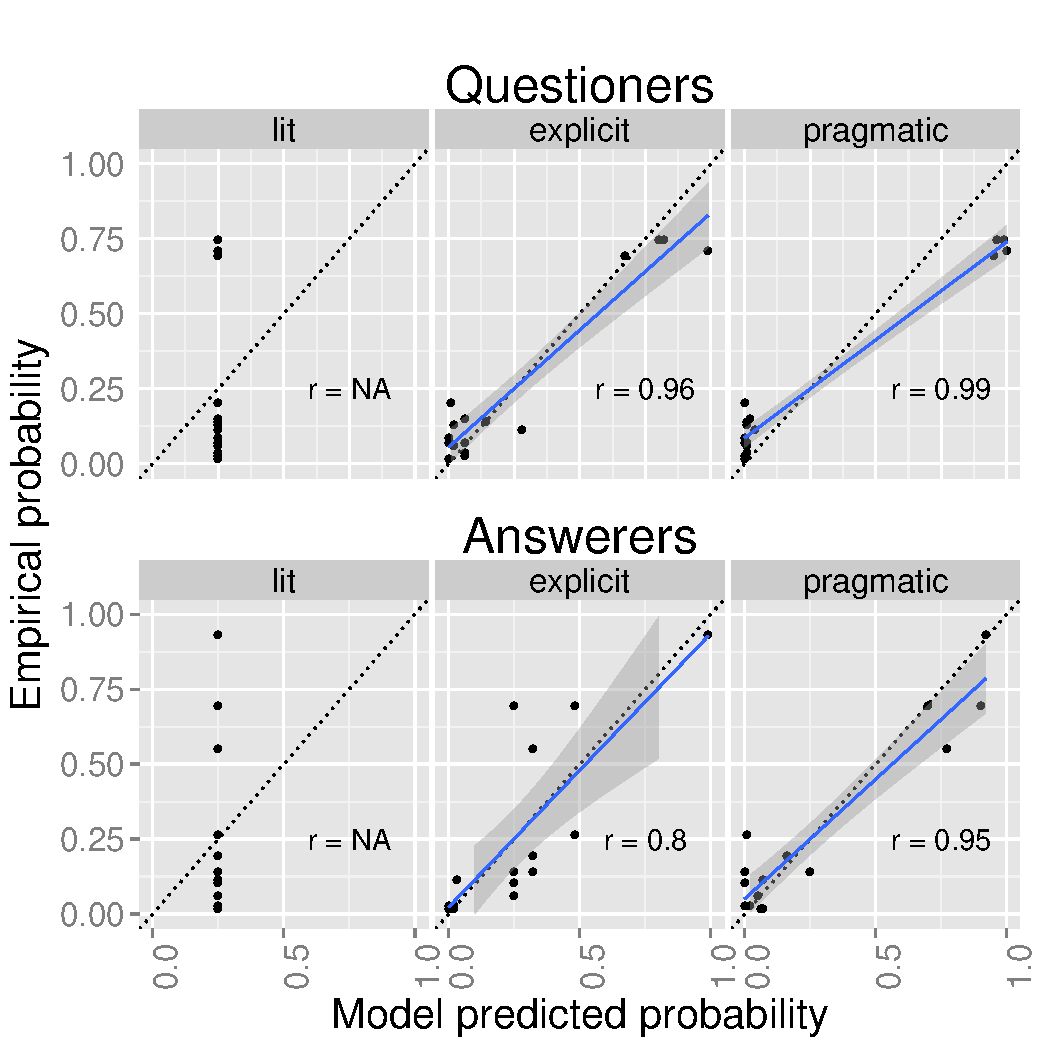
\includegraphics[scale=.45]{model_fits_grid.pdf}
\end{center}
\vspace{-.65cm}
\caption{Full space of models, and their correlations with the data from Exp.~1. Questioner models in the first row reason about the answerers directly below them, and the pragmatic answerer reasons about the explicit questioner.}
\label{fig:model_space}
\end{figure}

The best-fitting pragmatic questioner model's predictions for each response distribution are shown in Fig.~\ref{fig:exp1res} (left). Although the magnitude of its predictions are not in perfect alignment with the magnitude of the data (because it is strongly optimizing), it captures most of the interesting qualitative patterns of the data, particularly the modal responses. 

Finally, the pragmatic answerer provides a much better fit to the data than the explicit answerer. To ensure equal footing for model comparison, we restricted both models to a single optimality parameter, shared by all agents within the recursion.
%The model comparison here is more involved, since the explicit answerer does not depend on a questioner at all and therefore only has one parameter. We impose the same restriction on the pragmatic answerer as we applied to the pragmatic questioner, fitting one optimality parameter held in common between all answerer agents, and a second parameter for the internal questioner. 
Fitting yielded a model-data correlation of $r = 0.8$ for the explicit answerer and $r = 0.95$ for the pragmatic answerer. 

Only the pragmatic answerer can account for essential qualitative features of the response data. In particular, the explicit answerer predicts that participants will be equally likely to show the `dalmatian,' `poodle,' and `cat' when asked about a mammal. Instead, the data show a significant preference for revealing the cat, leaving `dalmatian' and `poodle' at the same level as the other alternative. The pragmatic answerer correctly predicts this pattern  (see Fig.~\ref{fig:exp1res} (left)). Even more dramatically, the explicit answerer predicts a uniform distribution over responses to the `animal?' question %(since all four responses denote animals)
. However, as shown by the $\chi^2$ tests above, the empirical distribution was significantly different from uniform. Thus, the pragmatic answerer is necessary to account for these data.

These data provide strong evidence for a pragmatic answerer, but are more equivocal with respect to the explicit and pragmatic questioner. Because the two models did not make significantly different predictions for this experiment (and both work quite well), we ran a follow-up study on a special case of the guessing-game paradigm in which the explicit and pragmatic questioners make different predictions.

\section{Exp.~2: A Critical Test of Questioner Models}

\subsubsection{Participants} We recruited 50 participants to participate only in the questioner scenario of the guessing game presented above. Ten participants were excluded on the basis of having a non-English native language, or reporting confusion about the instructions.

\subsubsection{Stimuli \& Procedure} The procedure was the same as before with some changes to the stimuli. The world space $\mathcal{W}$ consisted of possible assignments of the three pets to three gates. The possible goals $\mathcal{G}$ were the dalmatian and poodle (not the cat). The possible questions $\mathcal{G}$ were `dalmatian?' or `cat?'.  The possible answers $\mathcal{A}$ were the three gates. Each participant was given the two goals in a random order\footnote{The experiment is online at \url{http://cocolab.stanford.edu/cogsci2015/Q_and_A/experiment2/experiment2.html}}. 

\subsubsection{Results}

When the goal was to find the dalmatian, participants were significantly more likely to ask about the dalmatian than the cat, $\chi^2(1) = 12, p < 0.001$. When the goal was to find the poodle, participants were marginally more likely to ask about the cat than the dalmatian, $\chi^2(1) = 3.6, p = 0.058$. When looking only at the first of the two trials, the dalmatian result held, $\chi^2(1) = 14.4, p < 0.001$, but participants' preference for asking about the cat disappeared, $\chi^2(1) = 0.07, p = 0.79$. These results are shown in Fig.~\ref{fig:exp2res}.

\subsubsection{Model comparison}

The explicit questioner predicts that participants should have no preference for a question, given the `poodle' goal, since an explicit answerer would be equally unlikely to give the desired answer for both. The pragmatic questioner model, however, predicts that participants should prefer to ask about the cat. This is because the (internal) pragmatic answerer would reason that if the questioner was interested in the dalmatian, they would ask about the dalmatian; if they didn't, they must be interested in the other possible goal. 

The data are equivocal. Overall, the response distribution matches the predictions of the pragmatic model: questioners prefer to ask about the cat. However, the model predicts that the questioner will produce a very different response distribution if it does not take into account the full space of possible goals. Participants who received the `poodle' goal on the first trial appeared to behave more like explicit questioners, but this could be explained as an informational asymmetry: if they thought the poodle was the only goal (counter to the instructions), then asking about the dog would be consistent with the pragmatic model as well. We discuss other examples of sensitivity to the presentation of information below.

%\section{Related work}

%Our account of question and answer behavior ultimately converges on a similar solution as contemporary decision theoretic or game theoretic accounts in linguistics. These theories were a response to early work on question and answer semantics, which focused on the notion of informativeness. In Groenendijk \& Stokhof's \citeyear{GroenendijkStokhof84_SemanticsOfQuestions} theory of question and answer semantics, asking a question induces a partition over the space of possible worlds, where each cell of the partition corresponds to a possible answer. An answer, then, consists of eliminating cells in this partition, and the most useful answers are those that eliminate all relevant alternatives to the true world. However, as van Rooy \cite{VanRooy03_QuestioningDecisionProblems} and others \cite{Ginzburg95_ResolvingQuestions} have pointed out, this predicts that \emph{wh}-questions like ``Where can I buy an Italian newspaper?'' can only be fully resolved by exhaustively mentioning whether or not such a newspaper can be bought at each possible location. Clearly, this is not the case: a single nearby location would suffice. These theories also cannot account for other contextual variation in what counts as a useful answer, such as questions like ``where are you?'' 

% More recent theories have tried to fix these problems by introducing some consideration of the questioner's goals. van Rooy \citeyear{VanRooy03_QuestioningDecisionProblems}, for instance, formalizes these goals as a decision problem faced by the questioner. A useful answer under this decision theoretic account is one that maximizes the expected value of the questioner's decision problem. A useful question is one that induces a sufficiently fine-grained partition, optimally distinguishing the worlds relevant to the decision problem. While this framework elegantly accounts for the context-dependence and relevance-maximization of question and answer behavior, it assumes that the questioner's decision problem is known \emph{a priori} by the answerer. If this were the case, the act of asking questions would seem irrelevant: why wouldn't the answerer directly tell the questioner which action to take? 

\section{General discussion}
\label{sec:gd}


Perhaps the most important formal advance of the models considered here is to move the Rational Speech Act framework beyond interpretation of single utterances (in context), to consider the dynamics of simple dialogs (albeit consisting of a single question and its answer). 
Doing so requires replacing the immediate motive to convey true information with the more distant motive to provoke useful information from one's interlocutor. On the answerer side, sophisticated inference was required to account for the implicit interests of the questioner. This provides a useful connection to current game-theoretic and decision-theoretic models \cite{VogelBodoiaPottsJurafsky13_EmergenceGricean, VanRooy03_QuestioningDecisionProblems}, which also emphasize the importance of goals and speaker beliefs in communication but do not address the complex interplay of inference between questioner and answerer.

We have presented evidence that answerer behavior is best described by a pragmatic model that \emph{does} reason about questioner intentions, using the question utterance as a signal. The superiority of the pragmatic answerer behavior was robust across all conditions. Questioner behavior, however, seemed to be much more dependent on experience and instructions. For example, in another version of the experiment, we did not emphasize certain aspects of the game, such as the fact that the answerer knows about the restricted answer set and the fact that it might be helpful to think about what someone might think when hearing your question (prompting perspective-taking). These instructions reflect essential informational assumptions about the model and without these instructions, questioner behavior shifted more toward that predicted by the explicit model. Indeed, it appears that our sample contained a mixture of explicit and pragmatic questioners. This may be a product of our artificial game paradigm, or it may be reflective of real tendencies in language use.


\begin{figure}[t!]
\begin{center}
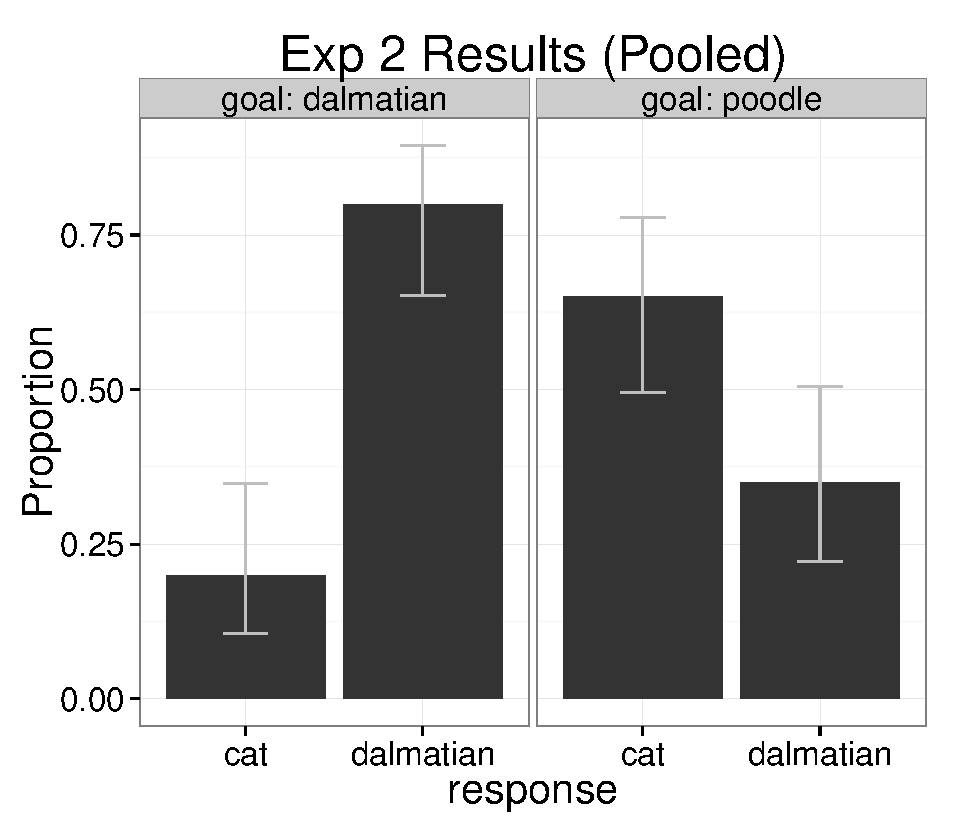
\includegraphics[scale=.235]{onlyPets_all.pdf}
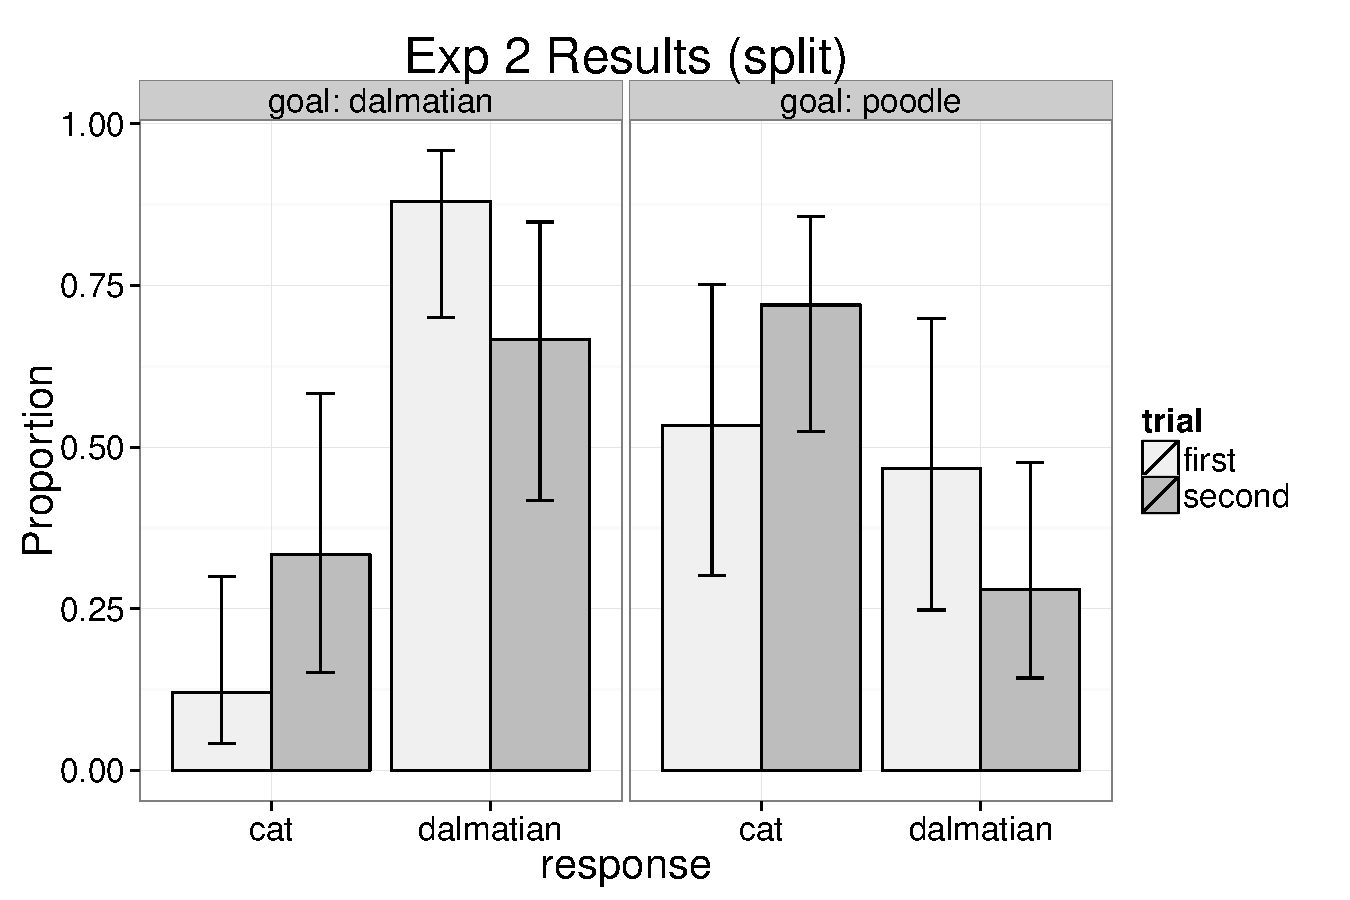
\includegraphics[scale=.235]{onlyPets_split.pdf}
\end{center}
\caption{The overall response distribution in Exp.~2 (left) and the same distribution split into first- and second-trial data (right).}
\label{fig:exp2res}
\end{figure}


While the artificiality of our experiment design seems to distance the behavior of participants from the types of questions and answers they would make using natural language, there are also some benefits to this design. First, it is easy to control the exact space of questions, goals, and answers, which is necessary for a first study of these phenomena. Moreover, while the restrictions on question space may seem peculiar, it is worth observing that many conversational scenarios in everyday usage also feature restrictions on the set of things one can ask about, due to politeness, salience, time cost, and other factors. In future work, we will explore the extent to which the proposed model can scale up to real-time, multiplayer games, extended dialogues, and other more naturalistic language settings. 

Humans are experts at inferring the intentions of other agents from their actions \cite{TomaselloCarpenter___Moll05_IntentionsCulturalCognition}. Given simple motion cues, for example, we are able to reliably discern high-level goals such as chasing, fighting, courting, or playing \cite{BarrettToddMillerBlythe05_IntentionFromMotionCues, HeiderSimmel44_ApparentBehavior}. Experiments in psycholinguistics have shown that this expertise extends to speech acts.  Behind every question lies a goal or intention. This could be an intention to obtain an explicit piece of information (``Where can I get a newspaper?''), signal some common ground (``Did you see the game last night?''), test the answerer's knowledge (``If I add these numbers together, what do I get?''), politely request the audience to take some action (``Could you pass the salt?''), or just to make open-ended small talk (``How was your weekend?''). These wildly different intentions seem to warrant different kinds of answers%, even if the explicit question is expressed using the same words
. By formalizing the computational process by which answerers infer these different intentions, our model framework provides a unifying way to accommodate this diversity.  % If questions themselves are informative, we must ask them carefully.


\bibliographystyle{apacite}

\setlength{\bibleftmargin}{.125in}
\setlength{\bibindent}{-\bibleftmargin}

\bibliography{bibs}


\end{document}
